\documentclass[12pt, titlepage]{article}
\usepackage{booktabs}
\usepackage{tabularx}
\usepackage{hyperref}
\usepackage{mdframed}
\usepackage{graphicx}
\usepackage{datetime}
\graphicspath{ {images/} }
\mdfsetup{nobreak=true}
\hypersetup{
    colorlinks,
    citecolor=black,
    filecolor=black,
    linkcolor=red,
    urlcolor=blue
}
\usepackage[round]{natbib}
\title{CS 4ZP6: Design Document
\\Cat and Mouse Game
\\ Revision 1}
\author{\textbf{Group \#08, ClawSome Games}
		\\ Yuan Gao (1330064)
		\\ Su Gao (1330065)
		\\ James Lee (1318125)
		\\ James Zhu (1317457) 
}
\newdate{date}{09}{04}{2017}
\date{\displaydate{date}}
\begin{document}
\maketitle
\pagenumbering{roman}
\tableofcontents
\listoftables
\listoffigures
\begin{table}[bp]
\caption{\bf Revision History}
\begin{tabularx}{\textwidth}{p{3cm}p{2cm}X}
\toprule {\bf Date} & {\bf Version} & {\bf Notes}\\
\midrule
11 Jan 2017 & 0 & Design Document 0\\
\midrule
9 April 2017 & 1 & Revised document according to feedback provided by Customer.\\
\bottomrule
\end{tabularx}
\end{table}
\newpage

\pagenumbering{arabic}

\section{Introduction}

\subsection{Overview}
\paragraph{}This document provides a detailed description of the design considerations and key methods and APIs which are used to implement the Cat-and-Mouse Game.




\section{Design Principle}
\subsection{A Component-Based Architecture}
\paragraph{}\textbf{The platform upon which we are developing The Cat-and-Mouse Game is the Unity 3D Game Engine, which utilises a component-based architecture.}
\paragraph{}Within this architecture, every component is encapsulated within the common GameObject class, which allows for
\paragraph{}This architecture facilitates fluidity and consistency between the various components of the game (eg. between the Heads Up Display (HUD) and the Physics System), such that, whilst still remaining a \textbf{discrete system} in of itself, each component within the system may interact with the other components in a stable and predictable manner through \textbf{established APIs}. 
\paragraph{}Thus, the \textbf{separation of concerns} which is enforced by the component based system enables for rapid prototyping and revision of the game, such that various objects and behaviours may be swapped in or out of the system with minimal impact on the operation of the overall system. This aspect is particularly useful in the construction of a system (such as a multiplayer game), which typically relies upon the composition of many small, independent systems, each performing a well-defined function.
\paragraph{}Furthermore, as this design pattern results in a system which exhibits \textbf{\emph{low coupling}} and \textbf{\emph{high cohesion}}, a highly parallel development life-cycle may be established, such that each component (or a set of related components--- such as the HUD and the Physics systems) may be developed in parallel, whilst minimising the risk for cross-contamination and lost development time.

\section{Anticipated Changes}

\subsection{Likely Changes}
\paragraph{}The following changes may occur during development of the project:
\paragraph{}AC1 The amount of features and types of objects will likely be increased during development. For example, currently there are only 5 types of power-ups, but we may increase this amount as we see fit for game balance and to increase user satisfaction.
\paragraph{}AC2 Modifications to how the characters interact with the environment are possible. Currently the player can only be blocked by walls but this may change if we decide that wall climbing or destructible terrain improves upon the user experience.
\paragraph{}AC3 The game modes system may also be changed, allowing multiple game modes such as a time based mode to be added, rather than only having the current kills based mode.
\paragraph{}AC4 Additional skills, abilities and actions that the players can perform will probably be added in the future.
\paragraph{}AC5 An increase in sound effects will likely be added.

\subsection{Unlikely Changes}
\paragraph{}The following changes are unlikely to occur during development of the project:
\paragraph{}UC1 The engine we use to develop the game, we will most likely stick to using the unity engine
\paragraph{}UC2 Currently the way networking is handled is by using the Photon Unity Network package. We will most likely not be changing the way networking is handled in our game
\paragraph{}UC3 The programming language used is C\# and will most likely stay that way.
\section{Module Interface Specification}
\subsection{Graphical User Interface (GUI)}
\paragraph{}In this selection, we discuss the Graphical User Interface components, including those belonging to the Menu and Heads-Up Display (HUD) Interfaces.
\subsubsection{COMPONENT: MainMenu}
\paragraph{}The MainMenu class allows the user to connect to the game server, set local game settings, as well as exit the game.
\begin{itemize}
    \item loadGame(): MainMenu \\ Connects to the game server and joins the Game Lobby.
    \item loadOptionsMenu(): MainMenu \\ Launches the Options Menu to allow the user to specific local settings (such as display options).
    \item ExitGame(): MainMenu \\ Terminates the program.
\end{itemize}
\subsubsection{COMPONENT: OptionsMenu}
\paragraph{}The Options Menu allows the user to specify local game settings.
\begin{itemize}
    \item setScreenResolution(): Integer$<$resolutionLevel$>$ \\ Sets the current display resolution (width x height), in pixels.
    \item setFullScreen(): Boolean$<$isFullScreen$>$ \\ Sets whether the game is displayed in Full Screen.
    \item setGraphicsSetting(): Integer $<$graphicsLevel$>$ \\ Sets the graphical quality in the game. Lower values increase performance whilst decreasing fidelity.
    \item setAudioEffectsLevel(): Integer$<$audioEffectsLevel$>$ \\ Sets the volume of the sound effects in the game.
    \item setAudioBackgroundLevel(): Integer$<$audioBackgroundLevel$>$  \\ Sets the volume of the background music in the game.
    \item setAudioEffectsMute(): Boolean$<$isAudioEffectsMuted$>$  \\ Sets whether the sound effects are muted in the game.
    \item setAudioBackgroundMute(): Boolean$<$isAudioBackgroundMuted$>$  \\ Sets whether the background music is muted in the game.
\end{itemize}
\subsubsection{COMPONENT: HUD}
\paragraph{}The Heads-Up Display (HUD) allows the user to view informationr regarding and trigger events which may change the state of the environment and/or other players.
\begin{itemize}
    \item activateSkill(): Integer$<$skillID$>$ \\ Activates the effects of a skill.
    \item updateDisplayHP(): Integer$<$currentHP$>$  \\ Updates the currently displayed Health Points of the player.
    \item updateDisplayMP(): Integer$<$currentMP$>$  \\ Updates the currently displayed Mana Points of the player.
    \item showPlayerStats(): HUD \\ Displays the current statistics (including Health, attributes and skills) of the player.
\end{itemize}
\subsubsection{COMPONENT: Skill}
\paragraph{}The skill module includes all the information about the abilities of the cat and mouse, such as skill name, cooldown, type, tier and so on. It includes many functions that allow the other classes to access the information, such as if the ability is on cooldown. It also updates the HUD in the Update() function when the user applies their skill points, so the skill will show up in the user's available skills.
This skill consists of a few small classes, such as the SkillSlot class, which handles a skill's images and indicators on the HUD, the CharSkill class, which handles the skill descriptions as well as it's attributes, and the main class Skill which includes the Start() function, Update() function, and various other helper functions.
\subsubsection{COMPONENT: Vitality}
\paragraph{}This component handles the character type, level, health points and experience points. It also displays the appropriate images for these elements, all in the bottom left corner of the HUD. The Update() function in this component constantly sets the indicators to the user's current statistics, so if the user takes damage the health bar will display the change immediately. The other helper functions such as setCurrentExperiencePoints() and getExp() are used by other classes to indicate changes towards the vitality system.
\subsection{Characters}
\paragraph{} In this section we discuss about the Character components, this includes the player controlled Mouse and Cat characters.
\subsubsection{COMPONENT: Cat}
\paragraph{} The Cat component handles everything related to the cat characters. These are user controlled characters that are in the team opposite of mouse characters. Cat characters have rigidbody components that are from Unity's scripting API, which allow them to be affected by Unity's physics engine. They also have colliders which handles collision detection.
\paragraph{} Scripts related to the Cat component include the CatCamMovement and CatMovement scripts. CatCamMovement handles camera controls for a cat, it also sets the position of the camera that follows the cat. CatMovement handles movement of the cat, it also handles functions such as ability use, jumping, and attacking.
\paragraph{} void Update() in CatCamMovement is where everything occurs, including acquiring inputs and transformation/rotation of the camera. The function void FixedUpdate() in CatMovement handles updating the GUI when health is lost, using abilites, movement, attacking, ability pickups, and jumping.
\subsubsection{COMPONENT: Mouse}
\paragraph{} The Mouse component is similar to the Cat component except it uses a different character model and colliders.
\paragraph{}Scripts relating to the mouse are MouseCamMovement for camera controls and positioning and also MouseMovement for movement controls and actions.
\paragraph{} void Update() in MouseCamMovement is where everything occurs, including acquiring inputs and transformation/rotation of the camera. The FixedUpdate() function does the same actions as the one in CatMovement.
\subsubsection{COMPONENT: Abilities}
\paragraph{} In this section we discuss the abilities component. Abilities, which also include powerups, are picked up on the map and are spawned by the map generation functions described in the Maze section below. Scripts and functions relating to how specific abilities work are under this component. These functions include void raiseHealth(), raiseMana(), raiseSpeed(), raiseJump(), isVisible(), raiseDamage(), doubleJump().
\paragraph{} The function raiseHealth() will increase a player's Health points by a fixed amount along with healing it. This will increase the value of the maxHealth variable. raiseMana() will increase a player's Mana points by a fixed amount, affecting the maxMana variable. raiseSpeed() will increase a character's movement speed, affecting the speed variable. raiseJump() will increase jumping height for a player and affect the jumpForce variable. raiseDamage() will increase a player's damage dealt when they attack and affect the attackPower variable. isVisible() allows users to become less visible for a set period of time. doubleJump() will allow users of the ability to jump twice before landing on the ground.
\subsubsection{COMPONENT: MonsterAI}
\paragraph{}This component handles the "brain" of the monsters in the maze. All the monsters use this same script, but they have different behaviours based on a variable \texttt{monsterType}. These monsters have 3 modes, sleeping (where they do nothing until they are attacked, upon which they switch to attack mode), patrol (where they walk aimlessly around the maze), and attack (where they follow and attack the closest player). This component handles all of the monster calculations, including attack chance, ability usage, switching of modes, and what to do when the monster is defeated. One major detail to note is that this component does not handle the movement of the monsters, it only sets the destination, as the NavMeshAgent (a built in component in Unity) will handle the movement of the monsters through the maze. 
The function setMonsterType() sets the monster type, playSound() plays the appropriate sound based on a type code and duration, and dealDamage() casts a sphere in front of the monster and deals damage to game objects hit. FixedUpdate() handles the animations of the monster, and Update() deals with the chances that the monster wlll attack or use abilities, as well as the timers until the monsters will change modes or until their abilities are off cooldown. 
\subsection{Maze}
\paragraph{} This section will be on Maze components, which creates the room and generates a maze.
\subsubsection{COMPONENT: Maze}
\paragraph{}In this section, we discuss the Maze component. 
\paragraph{} The CreateRoom() function creates a new room. Function StartMazeCreation() generates the maze, calling other functions in the process. These functions include the functions which generate the arches, doors, walls, and passages.
\subsection{Network}
\paragraph{} In this section we will be discussing the components that handle networking aspects of the game.
\subsubsection{COMPONENT: NetworkManager}
\paragraph{} The NetworkManager class is used to manage networking in this project. In it we can connect to servers, handle network events, and how scenes are created for clients. It syncs actions when multiple clients are connected so that events happening on the screen are the same, and the maze generated is also the same between players.
\paragraph{} void OnJoinedRoom() is that function that handles what events occur after joining a room.
\paragraph{} void SpawnCat(), void SpawnMouse(), and void SpawnMonster() are functions that can be called in OnJoinedRoom() in order to spawn players (cat or mouse) and monsters.
\section{Error Handling} 
\subsection{Missing Files}
\paragraph{}As the game is not distributed as contained within a single executable file, there will be many folders that will contain assets and libraries that the game will require to run. Should the game download was not complete, the user delete some files, or the downloaded files are incomplete or corrupt, then the game may not run properly (eg. result in missing textures, etc). Whilst having certain missing files will not stop the execution of the game, the absence of major components (such as files defining basic game behaviour) will cause the game to behave in unexpected ways and/or terminate.
\subsection{Library Initialization Failures}
\paragraph{}If the user does not have the required dependencies/libraries installed on their computer, then the game will terminate following an error message being displayed.
\subsection{Synchronization Errors}
\paragraph{}As a major component of the Cat-and-Mouse game requires a consistent Internet connection in order to implement the multiplayer capabilities, there will be many instances wherein many users will be present and interacting within a shared game session.
\paragraph{}This has the potential to give rise to synchronization errors, wherein there exists a discrepancy in the state of each user's game within the same session (eg. which may present itself as a variation in the positions of objects and players.)
\subsection{Unexpected Errors}
\paragraph{}Unexpected errors occurring is still a possibility, due to the potential for the game to enter states which are unaccounted for, as well as external factors within the environment in which the system will run, which is out of the control of the development team (such as hardware and/or operating system faults).

\section{User Interface Elements}
\subsection{User Interface}
\paragraph{}The Cat-and-Mouse game will consist of three main types of interfaces: \textbf{Menu Interfaces}, \textbf{Heads-Up Display (HUD) Interfaces}, and \textbf{Multiplayer Interaction Interfaces}.
\subsubsection{Menu Interfaces}
\paragraph{} Menu interfaces allow for the user to start and specify custom settings for the operation of the game on the client-side. This includes:
\begin{itemize}
    \item Starting and exiting a new instance of the game, termed a "client". \hyperref[fig:menu]{Figure~\ref*{fig:menu}} shows an interface capable of this.
    \item Customising audio, graphical, and other aspects of the user interface, on the client. \hyperref[fig:settings]{Figure~\ref*{fig:settings}} shows a menu interface with customization options for the game.
    \item Creating a new or joining an existing game session using the Multiplayer Interaction interfaces. 
\end{itemize}  

\subsubsection{HUD Interfaces}
\paragraph{}HUD Interfaces allow for the user to provide input using devices such as the keyboard and mouse, in order trigger certain events and thus affect the state of the game session. The HUD Interfaces also allow for the user to perceive output, as a result of these state changes. For instance, players may:
\begin{itemize}
    \item Activate a skill to affect one or more conditions and/or behaviours within the map
    \item Be notified on the current Health and Mana status of their character
    \item Be notified on the current locations and states of the other players within the map
    \item Send pre-defined, short messages to other users within the map
\end{itemize}
\paragraph{}An example HUD can be seen in \hyperref[fig:HUD]{Figure~\ref*{fig:HUD}}, where there are 3 buttons in the center indicating skills, a health bar to the left, and a minimap to the right.

\subsubsection{Multiplayer Interaction Interfaces}
\paragraph{} Multiplayer Interaction Interfaces allow for the user to create, connect to, and monitor the status of game sessions using the Photon Unity Networking Interface. Users may:
\begin{itemize}
    \item Create or join an online multiplayer game session hosted on the Photon Cloud Network. \hyperref[fig:lobby]{Figure~\ref*{fig:lobby}} shows an example of what this lobby will look like. 
    \item Select a map, team, and game mode for the multiplayer game session via consensus with other users within the game session. \hyperref[fig:select]{Figure~\ref*{fig:select}} shows an example of what this will look like. 
    \item View the profile information (eg. username) and current status of all users within the game session
\end{itemize}
\begin{figure}
    \centering
    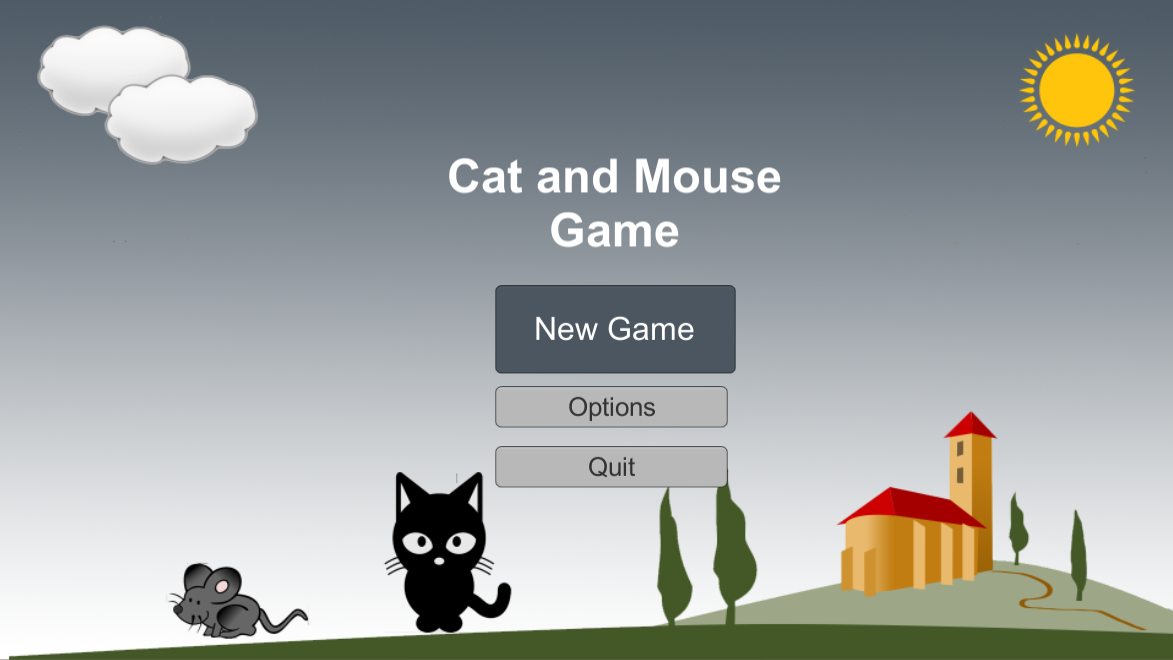
\includegraphics[width=1.00\textwidth]{menu}
    \caption{Example Start Screen}
    \label{fig:menu}
    \centering
    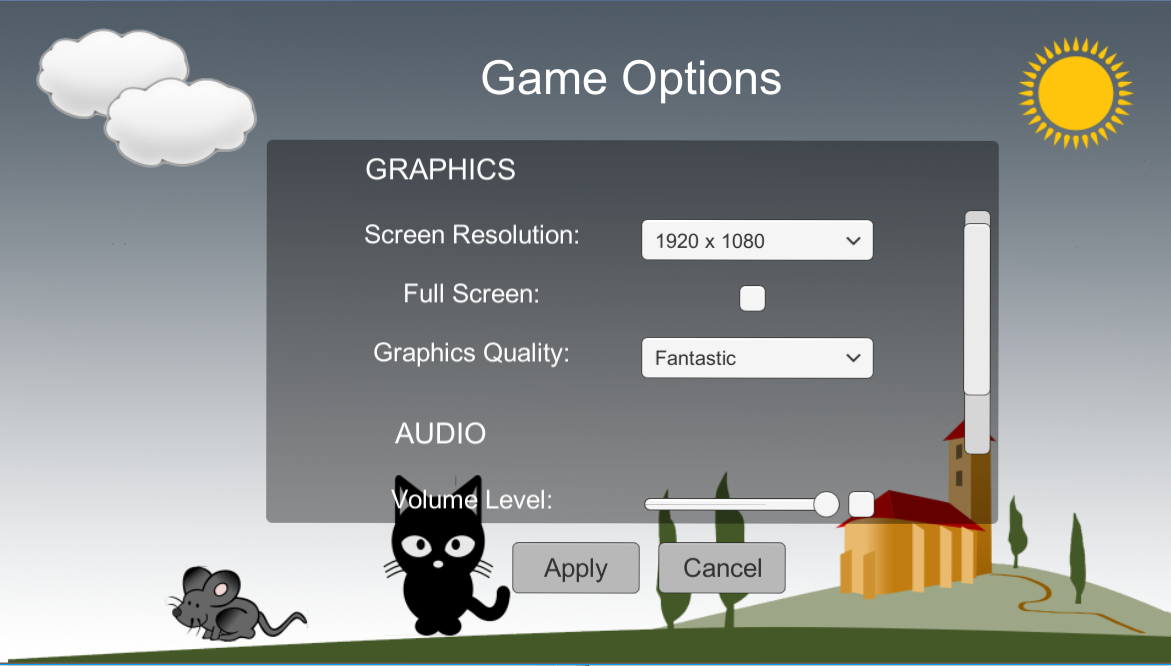
\includegraphics[width=1.00\textwidth]{settings}
    \caption{Example Settings Menu}
    \label{fig:settings}
\end{figure}
\begin{figure}
    \centering
    
\includegraphics[width=1.00\textwidth]{HUD}
    \caption{Example HUD}
    \label{fig:HUD}
\end{figure}
\begin{figure}
    \centering
    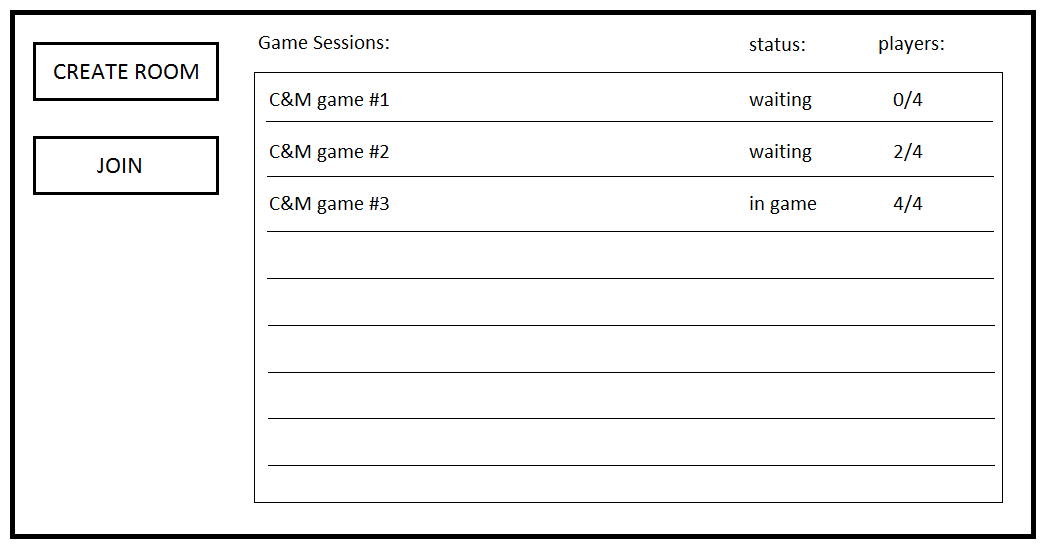
\includegraphics[width=1.00\textwidth]{lobby}
    \caption{Example Lobby}
    \label{fig:lobby}
\end{figure}
\begin{figure}
    \centering
    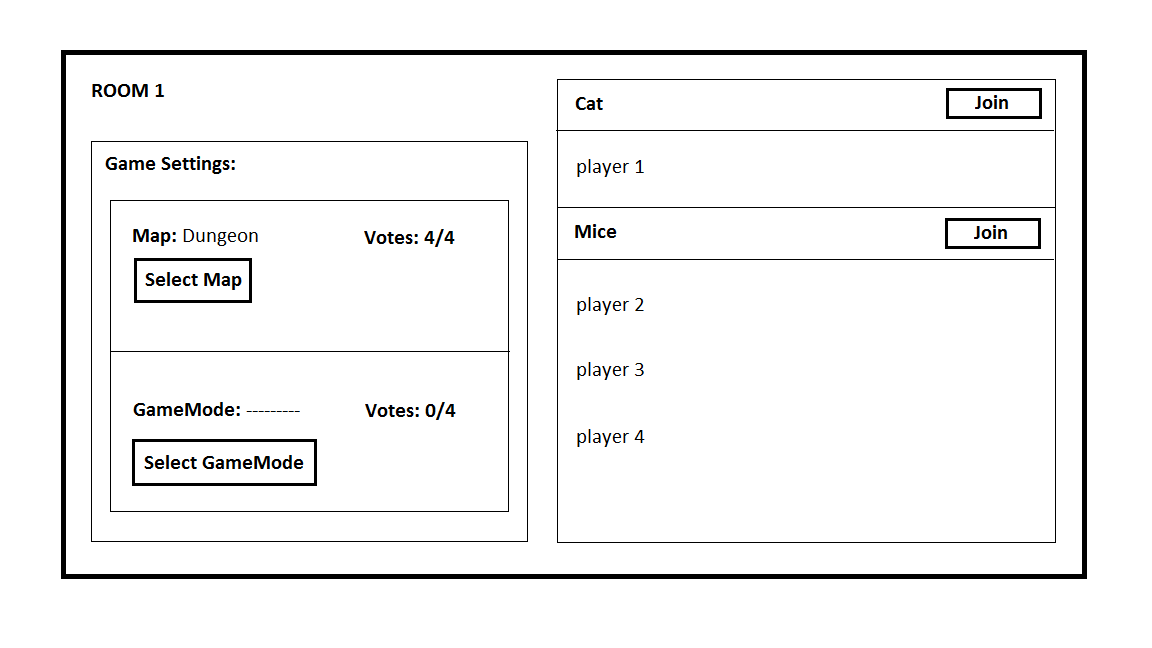
\includegraphics[width=1.00\textwidth]{select}
    \caption{Example Selection Menu}
    \label{fig:select}
\end{figure}
\section{Key Algorithms}
\paragraph{}There are many different algorithms used in the design of this game, ranging from maze generation to how each component interacts with other components and the environment. 
\subsection{The Maze Generation Algorithm}
\paragraph{}We wanted a maze that has no closed rooms, meaning that every room is accessible without climbing over or ignoring obstacles such as walls. To do this, we combined the use of many components and their partner scripts, and wrote an algorithm that generated lines of cells in random directions until all the cells in the predetermined space were filled in. Each cell is also created with walls which have directions assigned based on the direction of the cell creation. There were many types of cells, each with their own models such as a wall with a torch on it. After this, rooms were assigned to cells, and walls in between cells of the same room were culled. The next steps were to apply textures to all the cells, then to remove all the duplicate walls and arches that were created. Finally, special rooms were assigned based on how large each room was, with doors replacing the arches, and these so called "puzzle rooms" are modified to match their puzzle type. 
\paragraph{}The maze algorithm was also designed in a way that would allow the exact same maze to be generated every time, given a certain seed value. This was done by using functions involving Perlin noise, cell coordinates, and a "seed" value given for generating the maze. This way, during creation of a game lobby during run time, this seed value will be able to be easily passed onto each of the players to generate the same maze. 

\subsection{Monster AI Algorithm}
\paragraph{}Monsters are placed at specific locations of each map to begin the game with, and have varying modes based on the game state. Each mode corresponds to a different set of actions that the monster can perform. There are three states to the monster AI, attacking, patrolling, and sleeping. 
=\paragraph{}\textbf{Attacking:} In this state, the monster will attack a player based on two factors, whoever attacked it last, and how far that player is from it. If the player is not in attack range, the monster will chase the player down using a Unity provided pathfinding algorithm, the NavMesh agent. After a certain amount of time, if the monster has not been defeated, it will switch back to the next mode, Patrol.
\paragraph{}\textbf{Patrol:} In this mode, the monster will walk back and forth between two points, and if a player moves too close and alerts the monster, it will switch to attack mode. If the monster has not been interrupted after a certain amount of time or certain amount of cycles, then it will switch to the Sleeping mode.
\paragraph{}\textbf{Sleeping:} In this state, the monster does not move, and will not perform any actions unless woken up by a player attacking it. However, there will be a chance that the monster will wake up, into the Patrol mode. 
\subsection{Player Abilities}
\paragraph{}There will be many types of player abilities in this game, ranging from abilities that interact with other players, the player themselves, or even with the environment. There will be abilities shared between the cats and the mice, such as jumping or attacking, but there will also be special abilities that only the cat or only the mice will have. Even though every ability is unique, each ability will follow a general algorithm upon execution.
\paragraph{}Upon a key press, the algorithm will first check to see what type of player pressed the ability key. Next, it will see if the player currently has access to the ability, meaning that if the player has not currently "learned" the ability, it will not be available to them for use. If the ability has been learned, then the algorithm will check to see if the ability is off cooldown. If the ability is still going through it's cooldown, or recharging period, then the ability will not be used. If the ability is ready however, then the player will perform the ability. 
\paragraph{}If the ability causes interaction between the ability and other objects to occur, then a collision check is performed, looking through each object with a certain flag in the collision radius, and performing a certain action if a collision is detected. If not, then the appropriate action dealing with no collision is then taken. 

\section{Data Model and Storage}
\paragraph{} The Cat-and-Mouse Game does not store any permanent state data either locally or on the server regarding any users or existing/completed game sessions, outside of any currently active game sessions. Upon termination of the game session (when all clients within the Room have exited), any temporary data which may have been stored (termed "session data") is deleted.
\paragraph{}A limited amount of strictly\emph{ local} data may be stored on the user's system to maintain continuity of the user client between game sessions. This only includes settings which are fully localised and do not affect the behaviour of the game session on the server, such as audio or graphical settings.

\section{Communication Protocols}
\paragraph{} \textbf{The Cat-and-Mouse Game utilises the Photon Unity Networking (PUN) Interface to enable online multiplayer capabilities.}
\subsection{Photon Unity Networking (PUN) Interface}
\paragraph{} The PUN interface allows for users on instances of the game (termed "clients") to connect to a common game session, wherein they may be able to interact with each other via a shared game environment.
\subsubsection{Server}
\paragraph{}The PUN handles all interactions between game clients via a \textbf{Master Server}. The Master Server facilitates the establishment of connections with and transfer of data to and from all active clients, manages the allocation of different sessions of the game, as well as  ensures that the available network resources are being distributed equally amongst all clients.
\paragraph{}The first step a client must do when wishing to access a game session is to connect to the Master Server. The master server be neutral to any one particular game client, to prevent the termination of the game for \emph{all game clients} upon disconnection.
\paragraph{}The \textbf{Photon Cloud}, a global distributed network of servers provided by Exit Games, will be utilised as the Master Server for the Cat-and-Mouse Game.
\subsubsection{Game Lobby}
\paragraph{}The \textbf{game lobby} is which all of the clients are placed upon upon successful connection to the Master Server. 
\paragraph{}It allows for all clients to see all of the available game sessions (termed \textbf{Rooms}) which are currently active, as well as select a Room to join.
\subsubsection{Rooms}
\paragraph{}\textbf{Rooms} are each of the instances of the game which is currently running on the Master Server. Multiple clients (up to the maximum  on the number of players allowed within a game session) may be connected to any one room.
\paragraph{}Upon connection to the \textbf{Lobby} section of a Room, clients may specify a map environment, game mode, as well as other properties for the match. All clients within the Room must arrive at a consensus regarding these properties before a Match may be started.
\paragraph{}From this point on, the game state of all clients will be synchronised to the Master Server. Should the connection of any individual  client be terminated, their game session will be terminated as well.
\paragraph{}Upon the confirmation of the properties of a match, all clients will join a \textbf{Match}, a common environment (also termed a "map" which has been set accordingly. Players may interact with each other within the context of the Match through the triggering of events (\emph{eg. such as activating a skill}), which then updates the common state of the Room and synchronises with all its participating clients.

\section{Implementation Specifics}
\subsection{Platform}
\paragraph{}The Cat-and-Mouse Game is implemented on the Unity 3D Game Engine.
\paragraph{} The game supports computer systems running:
\begin{description}
    \item [Operating System:] Microsoft Windows, XP SP2 or higher
    \item [Graphics Card:] Supports DirectX 9 (Shader Model 3.0) 
    \textbf{\emph{or}} DirectX 11 DirectX feature level 9.3 support
    \item [CPU:] Supports the SSE2 instruction set
    \item [Input:] Keyboard and mouse
    \item [Networking:] Broadband Internet connection. Always online
\end{description}
\subsection{Language}
\paragraph{}The game is developed using the \textbf{C\# programming language.}
\subsection{Supporting Libraries}
\paragraph{}The game utilises the the following external packages and libraries (in addition to the core Unity 3D Engine):

\begin{table}[h]
\begin{tabularx}{\textwidth}{p{5cm}X}
    \toprule {\bf Package/Library} & {\bf Function}\\
    \midrule
    \href{https://www.photonengine.com/en/PUN}{Photon Unity Networking} & Unity 3D Package. Enables multiplayer capabilities through an online server.
    \bottomrule
\end{tabularx}
\caption{\textbf{External libraries and packages utilised by the Cat-and-Mouse Game}} \label{tab:libs}
\end{table}

\end{document}
